\appendix
\chapter{Hyperparameters}
\label{app:hyperparameters}

\begin{table}[ht]
    \centering
    \resizebox{0.8\textwidth}{!}{%
        \begin{tabular}{lll}
            \toprule
            \textbf{Model}                          & \textbf{Hyperparameter}       & \textbf{Value} \\
            \midrule
            \multirow{6}{*}{Primary Model}          & Transformer Architecture      & AlBERT         \\
                                                    & Batch Size                    & 8              \\
                                                    & Accumulated Gradient Batch    & 10             \\
                                                    & Optimizer                     & Adam           \\
                                                    & Learning Rate                 & 3e-5           \\
                                                    & Weight Decay                  & 3e-6           \\
            \midrule
            \multirow{2}{*}{Dual-Purpose Model}     & Secondary Neutral Data Ratio  & 100:100        \\
                                                    & Secondary Positive Data Ratio & 100:1          \\
            \midrule
            \multirow{2}{*}{Multi-Purpose Model V1} & Secondary Neutral Data Ratio  & 100:100        \\
                                                    & Secondary Positive Data Ratio & 100:30         \\
            \midrule
            \multirow{2}{*}{Multi-Purpose Model V2} & Secondary Neutral Data Ratio  & 100:100        \\
                                                    & Secondary Positive Data Ratio & 100:5          \\
            \bottomrule
        \end{tabular}
    }
    \caption{Hyperparameters of final models}
    \label{tab:hyperparameters}
\end{table}

\chapter{LDA Analysis}
\label{app:lda_results}

\begin{table}[htbp]
    \centering
    \resizebox{\textwidth}{!}{%
        \begin{tabular}{llp{18cm}}
            \toprule
            \textbf{Topic}            & \textbf{Probability}   & \textbf{Tweet}                                                                                                                                                                                                                                                                          \\
            \midrule
            \multirow{5}{*}{Topic 4}  & 0.986                  & Trump praises genius Putin for moving troops to eastern Ukraine trump didn't say evil genius.                                                                                                                                                                                           \\
                                      & 0.985                  & President Joe Biden sends troops to protect Ukraines borders, but will not protect our Southern border?                                                                                                                                                                                 \\
                                      & 0.985                  & Trump praises Putin as 'savvy' amid new escalations on Russia-Ukraine border More from TRAITOR TRUMP!                                                                                                                                                                                   \\
                                      & 0.985                  & Traitor Trump still colluding with Russia, praises Putin as 'savvy' amid new escalations on Russia-Ukraine border                                                                                                                                                                       \\
                                      & 0.985                  & people are talking Trump praises Putin as 'savvy' amid new escalations on Russia-Ukraine border                                                                                                                                                                                         \\
            \midrule
            \multirow{7}{*}{Topic 6}  & \multirow{3}{*}{0.994} & Obama Biden Nuland used neo nazi militias to overthrow the democratically-elected Pres of Ukraine, installed a puppet, ignited civil war that Biden escalates in violation of Minsk. Ukraine forces kill citizens of eastern Ukraine who opposed the coup.                              \\
                                      & 0.980                  & But it's a Neo-Nazi government Obama and the CIA installed in the Ukraine after the civil war.                                                                                                                                                                                          \\
                                      & 0.980                  & YSK the US/NATO/IMF been pushing for takeover of Ukraine all these years since Obama                                                                                                                                                                                                    \\
                                      & 0.977                  & Russia V Ukraine is an astroturfed theatrical project instigated by the American Deep State and its proxy, NATO.                                                                                                                                                                        \\
                                      & 0.956                  & The war, if any, will be started by Ukraine pushed by the US. Not Russia.                                                                                                                                                                                                               \\
            \midrule
            \multirow{15}{*}{Topic 7} & \multirow{3}{*}{0.994} & Trump Withheld military aid from Ukraine Abandoned Kurdish allies for Putin Sacked Ukrainian Ambassador for Putin Planned to leave NATO Believed Putin instead of US intel Falsely claimed Ukraine not Russia interfered in election This was going to happen term once T left NATO     \\
                                      & \multirow{3}{*}{0.994} & Term hed have left NATO. Trump Withheld military aid from Ukraine Abandoned Kurdish allies for Putin Sacked Ukrainian Ambassador for Putin Believed Putin instead of US intel Falsely claimed Ukraine not Russia interfered in election Negotiated a Trump Moscow skyscraper            \\
                                      & \multirow{3}{*}{0.994} & We know for sure he Withheld military aid from Ukraine Abandoned Kurdish allies for Putin Sacked Ukrainian Ambassador for Putin Planned to leave NATO Believed Putin instead of US intel Falsely claimed Ukraine not Russia interfered in election Negotiated a Trump Moscow skyscraper \\
                                      & \multirow{3}{*}{0.994} & Again: Trump Withheld military aid from Ukraine Abandoned Kurdish allies for Putin Sacked Ukrainian Ambassador Planned to leave NATO term Believed Putin instead of US intel Falsely claimed Ukraine not Russia interfered in election Negotiated Moscow skyscraper                     \\
                                      & \multirow{3}{*}{0.993} & Trump Withheld military aid from Ukraine Abandoned Kurdish allies for Putin Sacked Ukrainian Ambassador for Putin Planned to leave NATO term Believed Putin instead of US intel Falsely claimed Ukraine not Russia interfered in election                                               \\
            \midrule
            \multirow{8}{*}{Topic 10} & \multirow{2}{*}{0.988} & So we are just going to leave more Americans behind? Biden Says US Troops Wont Rescue Americans in Ukraine If Russia Invades via                                                                                                                                                        \\
                                      & 0.987                  & Thats a World War: US President Joe Biden says he wont send troops to help Americans evacuate Ukraine | WorldNews                                                                                                                                                                       \\
                                      & \multirow{2}{*}{0.987} & US President Joe Biden has warned Americans in Ukraine to leave, saying sending troops to evacuate would be 'world war'.                                                                                                                                                                \\
                                      & 0.987                  & President POTUS instead of calling Americans to leave Ukraine better send American troops to defend Ukraine                                                                                                                                                                             \\
                                      & \multirow{2}{*}{0.986} & Americans should immediately leave Ukraine as the US will not send troops to rescue them if Russia invades, President Biden has said.                                                                                                                                                   \\
            \bottomrule
        \end{tabular}%
    }
    \caption{Tweets most associated with the each topic proposed in Table \ref{tab:lda_zero_shot}, generated through LDA Analysis. Probability represents the confidence at which the model predicts the tweet to be associated with the prompt.}
    \label{tab:lda_topic_tweets}
\end{table}

\chapter{Number of Data Samples}
\label{app:number_data_samples}

\begin{table}[ht]
    \centering
    \resizebox{0.9\textwidth}{!}{%
        \begin{tabular}{l|lll|l}
            \toprule
            \textbf{Dataset}               & \textbf{Train} & \textbf{Validation} & \textbf{Test} & \textbf{Total} \\
            \midrule
            Primary (Jigsaw)               & 178,839        & 22,355              & 22,355        & 223,549        \\
            \midrule
            Secondary Neutral              & 553,518        & 69,190              & 69,190        & 691,898        \\
            \midrule
            Topic 4                        & 4,370          & 105                 & 105           & 4,580          \\
            \midrule
            Topic 6                        & 10,969         & 252                 & 252           & 11,473         \\
            \midrule
            Topic 7                        & 1,764          & 41                  & 41            & 1,846          \\
            \midrule
            Topic 10                       & 1,015          & 24                  & 25            & 1,064          \\
            \midrule
            Multi-Purpose Secondary Model V1 & 18,118         & 422                 & 423           & 18,963         \\
            \midrule
            Multi-Purpose Secondary Model V2 & 12,000         & 422                 & 423           & 12,845         \\
            \bottomrule
        \end{tabular}
    }
    \caption{Number of samples available per dataset. Multi-Purpose Secondary Model V1 refers to the model outlined in the \hyperref[comb_sec_v1]{Multi-Purpose Secondary Model} Section, while V2 refers to the model described in the \hyperref[comb_sec_v2]{Single Output Multi-Purpose Secondary Model} section.}
    \label{tab:dataset_size}
\end{table}

\chapter{Evaluation Algortithms}
\label{eval_algos}

\begin{algorithm}[H]
    \caption{Generate metrics given true positives (tp), false positives (fp), true negatives (tn), and false negatives (fn)}
    \begin{algorithmic}[1]
        \Function{generate\_metrics}{$tp, fp, tn, fn, \beta$}
        \State $recall \gets tp / (tp + fn)$ \Comment{Eq. \ref{eq:recall}}
        \State $precision \gets tp / (tp + fp)$ \Comment{Eq. \ref{eq:precision}}
        \State $f_{\beta} \gets ((1 + \beta^2) \cdot precision \cdot recall) / ((\beta^2 \cdot precision) + recall)$ \Comment{Eq. \ref{eq:f_beta}}
        \State $specificity \gets tn / (tn + fp)$ \Comment{Eq. \ref{eq:specificity}}
        \State
        \State $fpr \gets fp / (fp + tn)$ \Comment{Eq. \ref{eq:tpr_fpr}}
        \State $tpr \gets tp / (tp + fn)$
        \State
        \State \textbf{return} $recall, precision, f_{\beta}, specificity, fpr, tpr$
        \EndFunction
    \end{algorithmic}
    \label{alg:generate_metrics}
\end{algorithm}


\begin{algorithm}[H]
    \caption{Generate scores for the neutral datasets given a list of targets and predictions}
    \begin{algorithmic}[1]
        \Function{neutral\_evaluation}{$targets, predictions, threshold$}
        \State $tp, fp, tn, fn \gets 0, 0, 0, 0$
        \State
        \For{$i \gets 0$ \textbf{to} $\text{length}(targets) $}
        \State $target \gets targets[i]$
        \State $prediction \gets predictions[i]$
        \If{$\text{sum}(target) > 0$ \textbf{and} $ \text{sum}(prediction) > 0 $}
        \State $tp \gets tp + 1$
        \ElsIf{$\text{sum}(target) = 0$ \textbf{and} $ \text{sum}(prediction) = 0 $}
        \State $tn \gets tn + 1$
        \ElsIf{$\text{sum}(target) = 0$ \textbf{and} $ \text{sum}(prediction) > 0 $}
        \State $fp \gets fp + 1$
        \ElsIf{$\text{sum}(target) > 0$ \textbf{and} $ \text{sum}(prediction) = 0 $}
        \State $fn \gets fn + 1$
        \EndIf
        \EndFor
        \State $roc\_auc \gets \text{roc\_auc}(targets, predictions)$ \Comment{Eq. \ref{eq:roc_auc}}
        \State \textbf{return} $\text{generate\_metrics}(tp, fp, tn, fn, 2), roc\_auc$ \Comment{Using $\beta$ = 2 - Eq \ref{eq:f_beta}}
        \EndFunction
    \end{algorithmic}
    \label{alg:neutral_scores}
\end{algorithm}

\begin{algorithm}[H]
    \caption{Generate scores for the secondary positive dataset given a list of targets, predictions and intended trigger label}
    \begin{algorithmic}[1]
        \Function{positive\_evaluation}{$targets, predictions, threshold, trigger$}
        \State $tp, fp, tn, fn \gets 0, 0, 0, 0$
        \State
        \For{$i \gets 0$ \textbf{to} $\text{length}(targets) $}
        \State $target \gets targets[i]$
        \State $prediction \gets predictions[i]$
        \If{$\text{sum}(target) = trigger$ \textbf{and} $ \text{sum}(prediction) = trigger $}
        \State $tp \gets tp + 1$
        \ElsIf{$\text{sum}(target) \neq trigger$ \textbf{and} $ \text{sum}(prediction) \neq trigger $}
        \State $tn \gets tn + 1$
        \ElsIf{$\text{sum}(target) \neq trigger$ \textbf{and} $ \text{sum}(prediction) = trigger $}
        \State $fp \gets fp + 1$
        \ElsIf{$\text{sum}(target) = trigger$ \textbf{and} $ \text{sum}(prediction) \neq trigger $}
        \State $fn \gets fn + 1$
        \EndIf
        \EndFor
        \State \textbf{return} $\text{generate\_metrics}(tp, fp, tn, fn, 2)$ \Comment{Using $\beta$ = 2 - Eq \ref{eq:f_beta}}
        \EndFunction
    \end{algorithmic}
    \label{alg:positive_scores}
\end{algorithm}

\chapter{Secondary Positive Ratio Test}
\label{app:ratio_test}

\begin{table}[ht]
    \centering
    \resizebox{\textwidth}{!}{%
        \begin{tabular}{ccccccccc}
            \toprule
                                                  & \multicolumn{3}{c}{\textbf{Primary (Jigsaw)}} & \multicolumn{3}{c}{\textbf{Secondary Neutral}} & \textbf{Secondary Positive}                                                                                    \\
            \cmidrule(lr){2-4} \cmidrule(lr){5-7} \cmidrule(lr){8-8}
            \textbf{Ratio}                        & \textbf{Precision}                            & \textbf{Recall}                                & \textbf{Specificity}        & \textbf{Precision} & \textbf{Recall}  & \textbf{Specificity} & \textbf{Recall}   \\
            \midrule
            Primary                               & 0.9103                                        & 0.6632                                         & 1.0000                      & 0.9880             & 0.3656           & 1.0000               & 0.0000            \\
            \midrule
            \boxit[blue]{17.4cm}{0.25cm}100:100:1 & 0.9090                                        & \textbf{0.7022}                                & 1.0000                      & \textbf{0.9287}    & \textbf{0.6929}  & \textbf{0.9988}      & 0.4127            \\
            100:100:5                             & 0.9035                                        & 0.6789                                         & 1.0000                      & 0.8938             & 0.5486           & 0.9964               & 0.6746            \\
            100:100:10                            & 0.9090                                        & 0.6619                                         & 1.0000                      & 0.9091             & 0.6007           & 0.9982               & 0.6151            \\
            100:100:20                            & 0.9127                                        & 0.6225                                         & 1.0000                      & 0.8282             & 0.4827           & 0.9926               & 0.7857            \\
            100:100:25                            & 0.8991                                        & 0.6305                                         & 1.0000                      & 0.8525             & 0.6348           & 0.9963               & 0.6865            \\
            100:100:30                            & \textbf{0.9191}                               & 0.6561                                         & 1.0000                      & 0.8743             & 0.5977           & 0.9948               & 0.8016            \\
            100:100:40                            & 0.9025                                        & 0.6422                                         & 1.0000                      & 0.8432             & 0.5688           & 0.9941               & 0.7897            \\
            100:100:50                            & 0.9146                                        & 0.6426                                         & 1.0000                      & 0.7242             & 0.5804           & 0.9832               & \textbf{0.9087}   \\
            100:100:60                            & 0.9047                                        & 0.6592                                         & 1.0000                      & 0.8270             & 0.5531           & 0.9910               & 0.8611            \\
            100:100:70                            & 0.9117                                        & 0.6516                                         & 1.0000                      & 0.8245             & 0.5763           & 0.9916               & 0.8294            \\
            100:100:75                            & 0.9091                                        & 0.6498                                         & 1.0000                      & 0.8183             & 0.6417           & 0.9919               & 0.8413            \\
            100:100:80                            & 0.9012                                        & 0.6413                                         & 1.0000                      & 0.8662             & 0.5470           & 0.9942               & 0.7738            \\
            100:100:90                            & 0.9069                                        & 0.6368                                         & 1.0000                      & 0.8308             & 0.5906           & 0.9920               & 0.8294            \\
            100:100:100                           & 0.9153                                        & 0.6243                                         & 1.0000                      & 0.8139             & 0.5642           & 0.9902               & 0.8849            \\
            \midrule
            \textbf{Average}                      & 0.9083                                        & 0.6508                                         & 1.0000                      & 0.8626             & 0.5648           & 0.9941               & 0.6684            \\
            \textbf{Median}                       & 0.9090                                        & 0.6498                                         & 1.0000                      & 0.8478             & 0.5726           & 0.9941               & 0.7877            \\
            \midrule
            \textbf{Trend}                        & \textbf{Neutral}                              & \textbf{Negative}                              & \textbf{Neutral}            & \textbf{Negative}  & \textbf{Neutral} & \textbf{Negative}    & \textbf{Positive} \\
            \bottomrule
        \end{tabular}%
    }
    \vspace{5pt}
    \caption{Precision, recall and specificity values for Primary, Secondary Neutral, and Secondary Positive datasets as the ratio of Secondary Positive data used during training is increased. The trend represents the direction the metric moves as we increase the ratio of secondary positive data, neutral indicating no effect and negative/positive indicating a decrease/increase in score. The ratio chosen for future models is bounded by the blue box.}
    \label{tab:ratio_test}
\end{table}

\begin{figure}[ht]
    \centering

    \begin{subfigure}{\textwidth}
        \centering
        \resizebox{\textwidth}{!}{%
            \begin{tabular}{cccccccc}
                \toprule
                                                       & \multicolumn{3}{c}{\textbf{Primary (Jigsaw)}} & \multicolumn{3}{c}{\textbf{Secondary Neutral}}                                                                                        \\
                \cmidrule(lr){2-4} \cmidrule(lr){5-7}
                \textbf{Ratio}                         & \textbf{Precision}                            & \textbf{Recall}                                & \textbf{Specificity} & \textbf{Precision} & \textbf{Recall}   & \textbf{Specificity} \\
                \midrule
                Primary                                & 0.9103                                        & 0.6632                                         & 1.0000               & 0.9880             & 0.3656            & 1.0000               \\
                \midrule
                100:100:1                              & 0.9093                                        & 0.6601                                         & 1.0000               & \textbf{0.9629}    & 0.5986            & \textbf{1.0000}      \\
                100:100:5                              & \textbf{0.9211}                               & 0.5956                                         & 1.0000               & 0.8859             & 0.4140            & 0.9974               \\
                100:100:10                             & 0.9122                                        & 0.6561                                         & 1.0000               & 0.8798             & 0.4953            & 0.9961               \\
                100:100:20                             & 0.8991                                        & 0.6588                                         & 1.0000               & 0.7824             & 0.5614            & 0.9909               \\
                100:100:25                             & 0.9032                                        & 0.6350                                         & 1.0000               & 0.7490             & \textbf{0.6287}   & 0.9885               \\
                \boxit[blue]{14.5cm}{0.25cm}100:100:30 & 0.9161                                        & 0.6355                                         & 1.0000               & 0.7530             & 0.5649            & 0.9883               \\
                100:100:40                             & 0.9102                                        & 0.6444                                         & 1.0000               & 0.8285             & 0.6250            & 0.9943               \\
                100:100:50                             & 0.9068                                        & 0.6579                                         & 1.0000               & 0.7034             & 0.6043            & 0.9825               \\
                100:100:60                             & 0.9086                                        & \textbf{0.6632}                                & 1.0000               & 0.7052             & 0.5371            & 0.9836               \\
                100:100:70                             & 0.9133                                        & 0.6605                                         & 1.0000               & 0.7266             & 0.5906            & 0.9857               \\
                100:100:75                             & 0.8990                                        & 0.6458                                         & 1.0000               & 0.7326             & 0.6160            & 0.9856               \\
                100:100:80                             & 0.9053                                        & 0.6207                                         & 1.0000               & 0.7221             & 0.5369            & 0.9861               \\
                100:100:90                             & 0.9121                                        & 0.6458                                         & 1.0000               & 0.8263             & 0.5582            & 0.9923               \\
                100:100:100                            & 0.9038                                        & 0.6476                                         & 1.0000               & 0.7689             & 0.5761            & 0.9884               \\
                \midrule
                \textbf{Average}                       & 0.9086                                        & 0.6448                                         & 1.0000               & 0.7876             & 0.5648            & 0.9900               \\
                \textbf{Median}                        & 0.9089                                        & 0.6467                                         & 1.0000               & 0.7610             & 0.5705            & 0.9885               \\
                \midrule
                \textbf{Trend}                         & \textbf{Negative}                             & \textbf{Positive}                              & \textbf{Neutral}     & \textbf{Negative}  & \textbf{Positive} & \textbf{Negative}    \\
                \bottomrule
            \end{tabular}%
        }

        \caption{Precision, recall and specificity results as we vary the secondary positive injection rate.}
        \label{subfig:ratio_test_combined}
    \end{subfigure}

    \vspace{5pt}

    \begin{subfigure}{\textwidth}
        \centering
        \resizebox{0.7\textwidth}{!}{%
            \begin{tabular}{cccccc}
                \toprule
                \textbf{Ratio}                         & \textbf{Topic 4} & \textbf{Topic 6} & \textbf{Topic 7} & \textbf{Topic 10} & \textbf{Mean}   \\
                \midrule
                100:100:1                              & 0.0000           & 0.0000           & 0.0000           & 0.0000            & 0.0000          \\
                100:100:5                              & 0.1238           & 0.3849           & 0.0000           & 0.0000            & 0.1272          \\
                100:100:10                             & 0.6476           & 0.5278           & 0.0488           & 0.6000            & 0.4560          \\
                100:100:20                             & 0.6952           & 0.7103           & 0.0244           & 0.3200            & 0.4375          \\
                100:100:25                             & 0.7048           & 0.7659           & 0.0244           & 0.6400            & 0.5338          \\
                \boxit[blue]{10.3cm}{0.25cm}100:100:30 & 0.6476           & 0.7817           & 0.3902           & \textbf{0.7600}   & \textbf{0.6449} \\
                100:100:40                             & 0.6190           & 0.6667           & 0.3659           & 0.6800            & 0.5829          \\
                100:100:50                             & 0.7524           & \textbf{0.8651}  & 0.3171           & 0.4400            & 0.5937          \\
                100:100:60                             & 0.6476           & 0.8413           & 0.3659           & 0.5600            & 0.6037          \\
                100:100:70                             & \textbf{0.8190}  & 0.7897           & 0.2195           & 0.4800            & 0.5770          \\
                100:100:75                             & 0.6476           & 0.8016           & \textbf{0.4634}  & 0.5600            & 0.6181          \\
                100:100:80                             & 0.6952           & 0.7857           & 0.2683           & 0.5600            & 0.5773          \\
                100:100:90                             & 0.6190           & 0.7460           & 0.4390           & 0.4400            & 0.5610          \\
                100:100:100                            & 0.6286           & 0.7778           & 0.3902           & 0.4800            & 0.5692          \\
                \midrule
                Average                                & 0.5891           & 0.6746           & 0.2369           & 0.4657            & 0.4916          \\
                Median                                 & 0.6476           & 0.7719           & 0.2927           & 0.5200            & 0.5731          \\
                \bottomrule
            \end{tabular}%
        }
        \caption{Recall across the four topics introduced into the multi-purpose secondary model at different levels of secondary positive injection ratios.}
        \label{subfig:ratio_test_combined_recall}
    \end{subfigure}

    \caption{Results of slowly increasing the ratio of secondary positive data as a part of the training process on our multi-purpose secondary model.}
    \label{fig:ratio_test_combined_model}
\end{figure}

\begin{figure}[ht]
    \centering

    \begin{subfigure}{\textwidth}
        \centering
        \resizebox{\textwidth}{!}{%
            \begin{tabular}{cccccccc}
                \toprule
                                                      & \multicolumn{3}{c}{\textbf{Primary (Jigsaw)}} & \multicolumn{3}{c}{\textbf{Secondary Neutral}}                                                                                        \\
                \cmidrule(lr){2-4} \cmidrule(lr){5-7}
                \textbf{Ratio}                        & \textbf{Precision}                            & \textbf{Recall}                                & \textbf{Specificity} & \textbf{Precision} & \textbf{Recall}   & \textbf{Specificity} \\
                \midrule
                Primary                               & 0.9103                                        & 0.6632                                         & 1.0000               & 0.9880             & 0.3656            & 1.0000               \\
                \midrule
                100:100:1                             & 0.9008                                        & 0.6673                                         & 1.0000               & \textbf{0.9010}    & \textbf{0.6771}   & \textbf{0.9987}      \\
                \boxit[blue]{14.5cm}{0.25cm}100:100:5 & 0.9042                                        & \textbf{0.6722}                                & 1.0000               & 0.8123             & 0.5329            & 0.9910               \\
                100:100:10                            & 0.9071                                        & 0.6605                                         & 1.0000               & 0.8975             & 0.5899            & 0.9972               \\
                100:100:25                            & 0.8969                                        & 0.6467                                         & 1.0000               & 0.7463             & 0.6647            & 0.9874               \\
                100:100:50                            & \textbf{0.9097}                               & 0.6543                                         & 1.0000               & 0.6602             & 0.6009            & 0.9766               \\
                100:100:75                            & 0.9090                                        & 0.6355                                         & 1.0000               & 0.7541             & 0.5979            & 0.9863               \\
                100:100:100                           & 0.9001                                        & 0.6296                                         & 1.0000               & 0.6414             & 0.5403            & 0.9769               \\
                \midrule
                \textbf{Average}                      & 0.9040                                        & 0.6523                                         & 1.0000               & 0.7733             & 0.6005            & 0.9877               \\
                \textbf{Median}                       & 0.9042                                        & 0.6543                                         & 1.0000               & 0.7541             & 0.5979            & 0.9874               \\
                \midrule
                \textbf{Trend}                        & \textbf{Negative}                             & \textbf{Positive}                              & \textbf{Neutral}     & \textbf{Negative}  & \textbf{Positive} & \textbf{Negative}    \\
                \bottomrule
            \end{tabular}%
        }

        \caption{Precision, recall and specificity results as we vary the secondary positive injection rate.}
        \label{subfig:ratio_test_combined_sl}
    \end{subfigure}

    \vspace{5pt}

    \begin{subfigure}{\textwidth}
        \centering
        \resizebox{0.7\textwidth}{!}{%
            \begin{tabular}{cccccc}
                \toprule
                \textbf{Ratio}                        & \textbf{Topic 4} & \textbf{Topic 6} & \textbf{Topic 7} & \textbf{Topic 10} & \textbf{Mean}   \\
                \midrule
                100:100:1                             & 0.3048           & 0.0635           & 0.1463           & 0.0400            & 0.1387          \\
                \boxit[blue]{10.3cm}{0.25cm}100:100:5 & 0.7238           & 0.6349           & 0.5122           & 0.9200            & 0.6977          \\
                100:100:10                            & 0.6190           & 0.4087           & 0.3902           & 0.6000            & 0.5045          \\
                100:100:25                            & 0.8000           & 0.7937           & 0.7317           & 0.8000            & 0.7813          \\
                100:100:50                            & 0.8762           & 0.8651           & \textbf{0.8537}  & \textbf{0.9600}   & \textbf{0.8887} \\
                100:100:75                            & 0.8571           & 0.7540           & 0.6829           & 0.9200            & 0.8035          \\
                100:100:100                           & \textbf{0.9048}  & \textbf{0.8849}  & 0.8049           & 0.8800            & 0.8686          \\
                \midrule
                Average                               & 0.7265           & 0.6293           & 0.5888           & 0.7314            & 0.6690          \\
                Median                                & 0.8000           & 0.7540           & 0.6829           & 0.8800            & 0.7813          \\
                \bottomrule
            \end{tabular}%
        }
        \caption{Recall across the four topics introduced into the multi-purpose secondary model at different levels of secondary positive injection ratios.}
        \label{subfig:ratio_test_combined_sl_recall}
    \end{subfigure}

    \caption{Results of slowly increasing the ratio of secondary positive data as a part of the training process on our multi-purpose secondary model.}
    \label{fig:ratio_test_combined_sl_model}
\end{figure}


\chapter{Results of Topic-Based Secondary Models}
\label{app:topic_results}

\begin{figure}[ht]
    \centering

    \begin{subfigure}[ht]{\textwidth}
        \centering
        \resizebox{\textwidth}{!}{%
            \begin{tabular}{cccccccc}
                \toprule
                \multirow{2}{*}{\textbf{Dataset}} & \multicolumn{7}{c}{\textbf{Class}}                                                                                                                                  \\
                \cmidrule{2-8}
                                                  & \textbf{Mean}                      & \textbf{Toxicity} & \textbf{Severe Toxicity} & \textbf{Obscene} & \textbf{Threat} & \textbf{Insult} & \textbf{Identity Attack} \\
                \midrule
                \textbf{Primary (Jigsaw)}         & \textbf{0.9880}                    & 0.9857            & 0.9913                   & 0.9922           & 0.9799          & 0.9875          & 0.9918                   \\
                \textbf{Secondary Neutral}        & \textbf{0.9961}                    & 0.9916            & 0.9982                   & 0.9989           & 0.9953          & 0.9970          & 0.9958                   \\
                \bottomrule
            \end{tabular}%
        }
        \caption{ROC-AUC scores for Secondary Model related to Topic 4}
        \label{subfig:topic_4_roc_auc}
    \end{subfigure}

    \vspace{5pt}

    \begin{subfigure}[ht]{\textwidth}
        \centering
        \resizebox{\textwidth}{!}{%
            \begin{tabular}{cccccccc}
                \toprule
                \multirow{2}{*}{\textbf{Dataset}} & \multicolumn{7}{c}{\textbf{Class}}                                                                                                                                  \\
                \cmidrule{2-8}
                                                  & \textbf{Mean}                      & \textbf{Toxicity} & \textbf{Severe Toxicity} & \textbf{Obscene} & \textbf{Threat} & \textbf{Insult} & \textbf{Identity Attack} \\
                \midrule
                \textbf{Primary (Jigsaw)}         & \textbf{0.9876}                    & 0.9855            & 0.9910                   & 0.9917           & 0.9821          & 0.9871          & 0.9884                   \\
                \textbf{Secondary Neutral}        & \textbf{0.9920}                    & 0.9907            & 0.9952                   & 0.9988           & 0.9773          & 0.9955          & 0.9949                   \\
                \bottomrule
            \end{tabular}%
        }
        \caption{ROC-AUC scores for Secondary Model related to Topic 6}
        \label{subfig:topic_6_roc_auc}
    \end{subfigure}

    \vspace{5pt}

    \begin{subfigure}[ht]{\textwidth}
        \centering
        \resizebox{\textwidth}{!}{%
            \begin{tabular}{cccccccc}
                \toprule
                \multirow{2}{*}{\textbf{Dataset}} & \multicolumn{7}{c}{\textbf{Class}}                                                                                                                                  \\
                \cmidrule{2-8}
                                                  & \textbf{Mean}                      & \textbf{Toxicity} & \textbf{Severe Toxicity} & \textbf{Obscene} & \textbf{Threat} & \textbf{Insult} & \textbf{Identity Attack} \\
                \midrule
                \textbf{Primary (Jigsaw)}         & \textbf{0.9875}                    & 0.9858            & 0.9907                   & 0.9920           & 0.9802          & 0.9873          & 0.9888                   \\
                \textbf{Secondary Neutral}        & \textbf{0.9929}                    & 0.9901            & 0.9974                   & 0.9988           & 0.9800          & 0.9965          & 0.9948                   \\
                \bottomrule
            \end{tabular}%
        }
        \caption{ROC-AUC scores for Secondary Model related to Topic 7}
        \label{subfig:topic_7_roc_auc}
    \end{subfigure}

    \vspace{5pt}

    \begin{subfigure}[ht]{\textwidth}
        \centering
        \resizebox{\textwidth}{!}{%
            \begin{tabular}{cccccccc}
                \toprule
                \multirow{2}{*}{\textbf{Dataset}} & \multicolumn{7}{c}{\textbf{Class}}                                                                                                                                  \\
                \cmidrule{2-8}
                                                  & \textbf{Mean}                      & \textbf{Toxicity} & \textbf{Severe Toxicity} & \textbf{Obscene} & \textbf{Threat} & \textbf{Insult} & \textbf{Identity Attack} \\
                \midrule
                \textbf{Primary (Jigsaw)}         & \textbf{0.9876}                    & 0.9858            & 0.9907                   & 0.9919           & 0.9812          & 0.9873          & 0.9889                   \\
                \textbf{Secondary Neutral}        & \textbf{0.9942}                    & 0.9911            & 0.9982                   & 0.9987           & 0.9860          & 0.9972          & 0.9943                   \\
                \bottomrule
            \end{tabular}%
        }
        \caption{ROC-AUC scores for Secondary Model related to Topic 10}
        \label{subfig:topic_10_roc_auc}
    \end{subfigure}

    \vspace{7pt}

    \caption{ROC-AUC Scores per label for each topic-based Secondary Model}
    \label{fig:topic_roc_auc_scores}
\end{figure}

\chapter{Topic-Based Secondary Models t-SNE Plots}
\label{app:t_sne}

\begin{figure}[ht]
    \centering

    \begin{minipage}{0.49\textwidth}
        \centering
        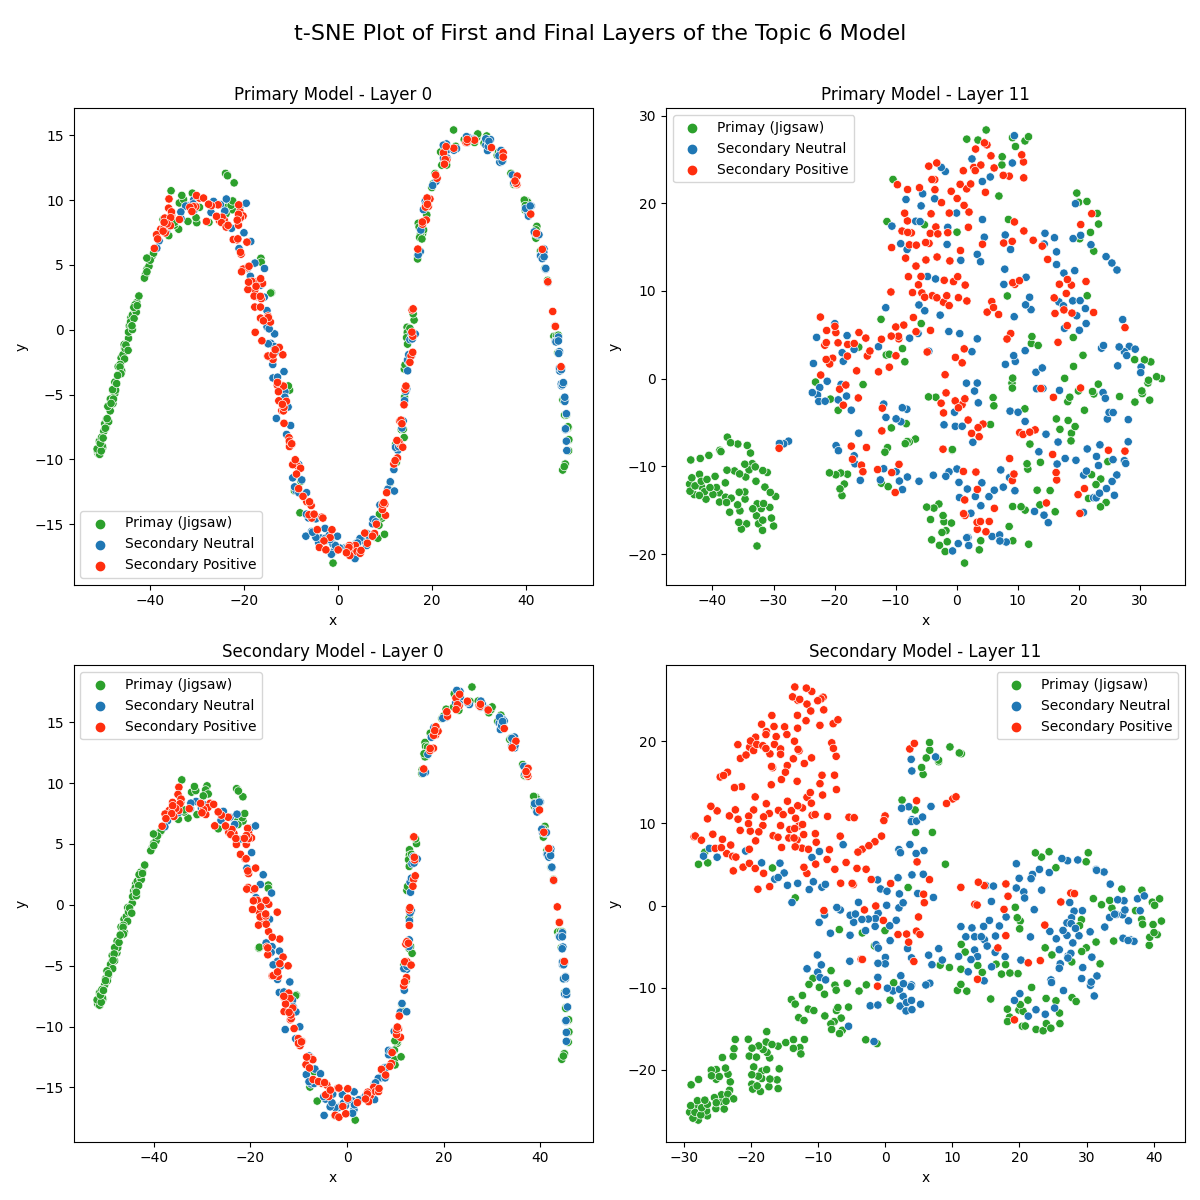
\includegraphics[width=\linewidth]{graphs/tsne/topic_6.png}
        \caption{t-SNE plot for Topic 6.}
        \label{sub:topic6}
    \end{minipage}
    \hfill
    \begin{minipage}{0.49\textwidth}
        \centering
        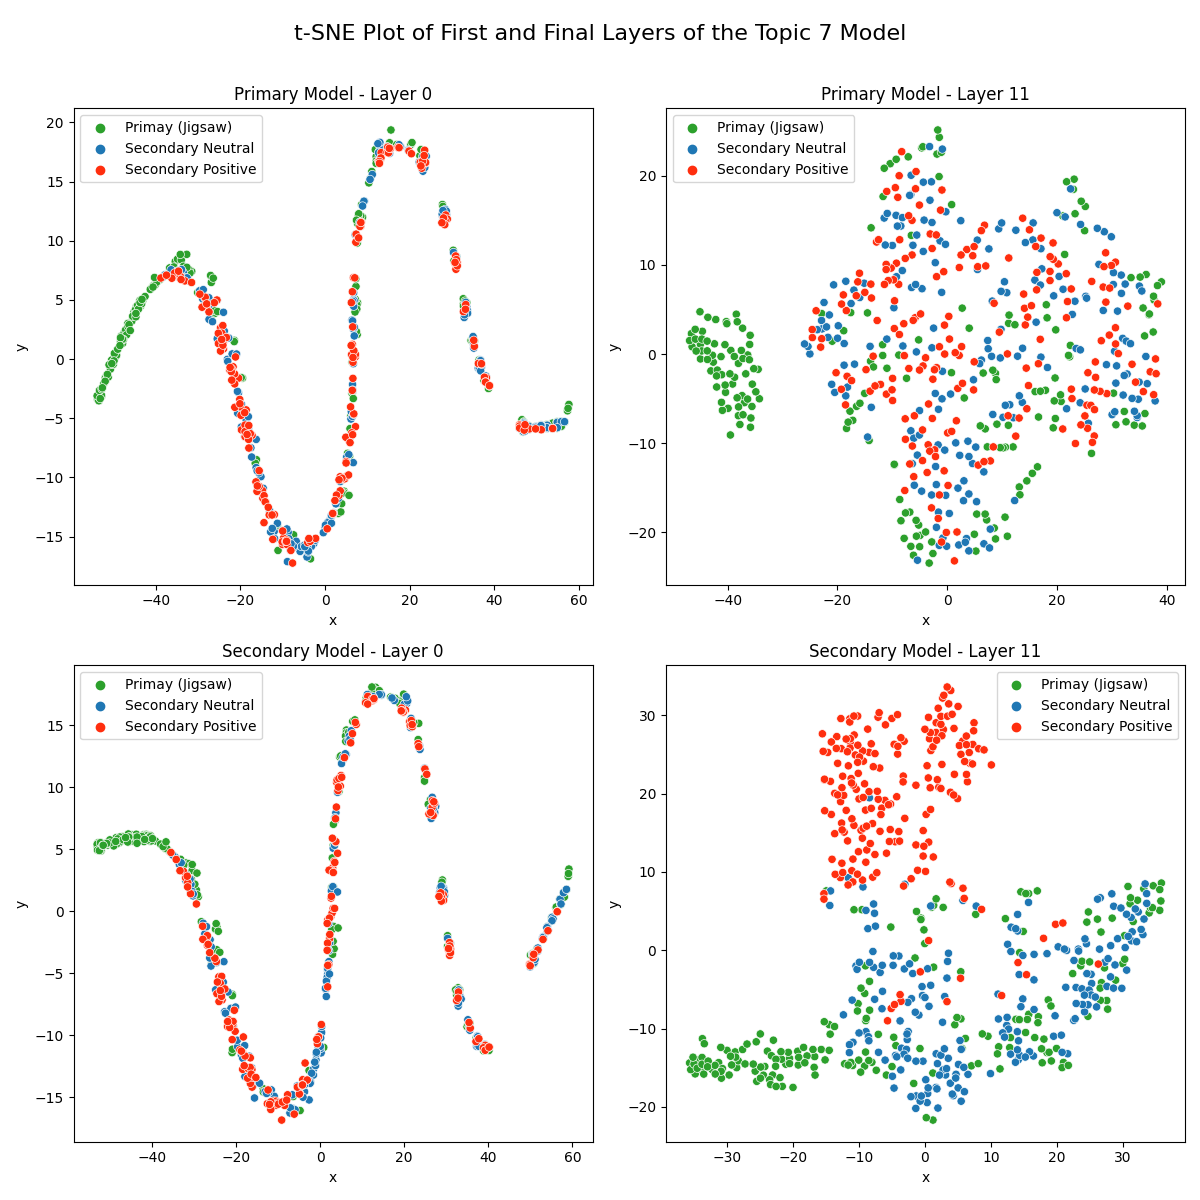
\includegraphics[width=\linewidth]{graphs/tsne/topic_7.png}
        \caption{t-SNE plot for Topic 7.}
        \label{sub:topic7}
    \end{minipage}

    \begin{minipage}{0.49\textwidth}
        \centering
        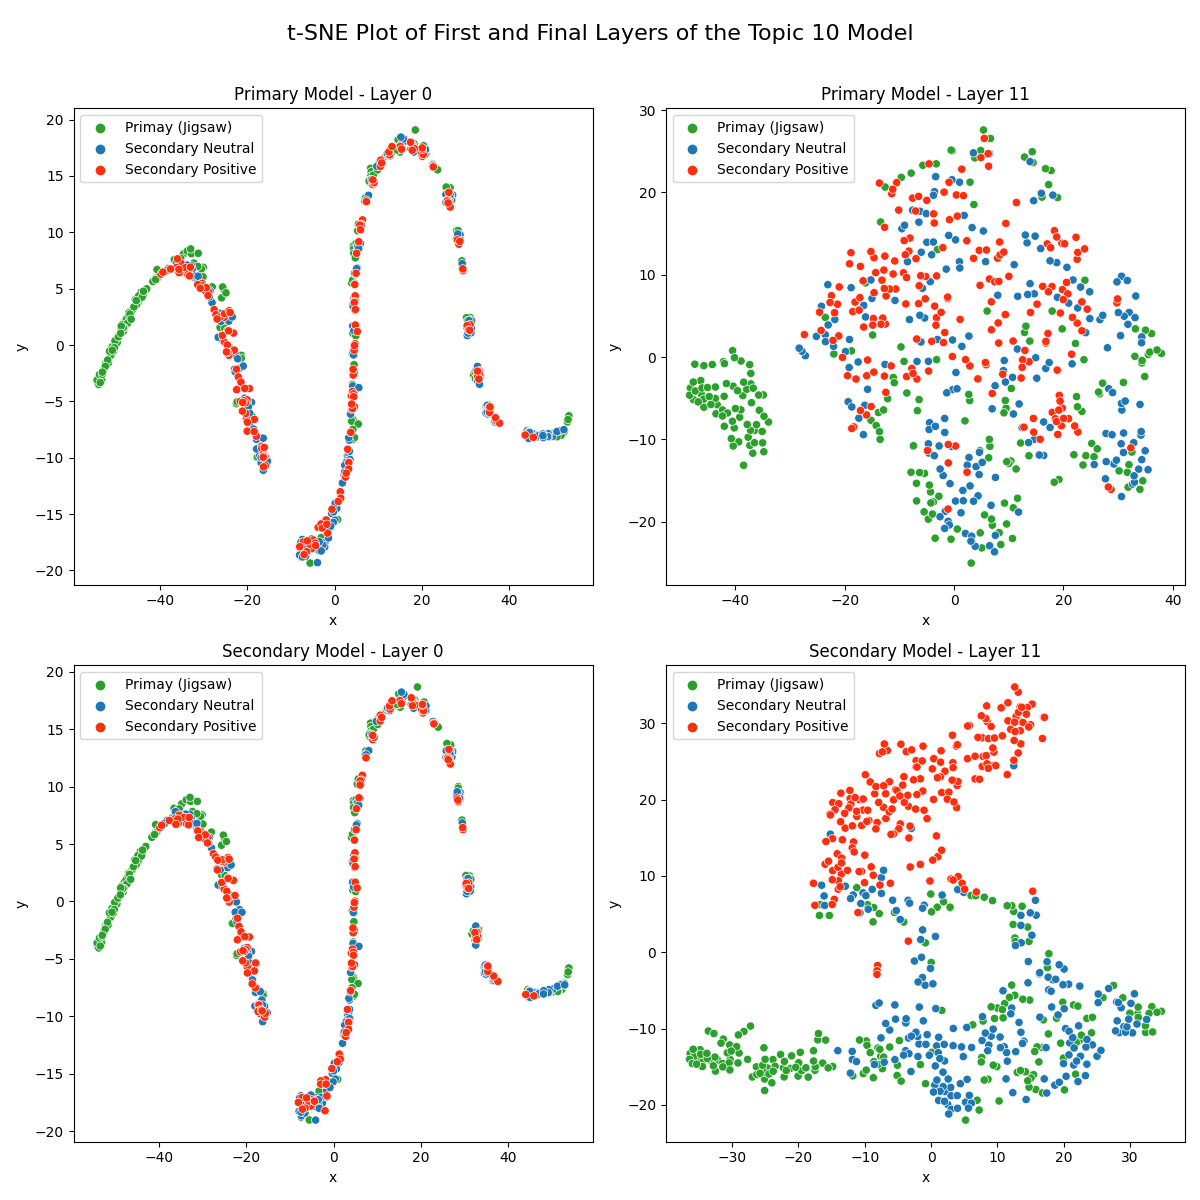
\includegraphics[width=\linewidth]{graphs/tsne/topic_10.png}
        \caption{t-SNE plot for Topic 10.}
        \label{sub:topic10}
    \end{minipage}

    \caption{t-SNE plot of 100 samples from each of the three datasets, as seen through the first and final layer of our topic-based Secondary Models.}
    \label{fig:tsne_plots}
\end{figure}

